%%%%%%%%%%%%%%%%%%%%%%%%%%%%%%%%%%%%%%%%%%%%%%%%%%%%%%%%%%%%%%%
%
% Welcome to writeLaTeX --- just edit your LaTeX on the left,
% and we'll compile it for you on the right. If you give 
% someone the link to this page, they can edit at the same
% time. See the help menu above for more info. Enjoy!
%
%%%%%%%%%%%%%%%%%%%%%%%%%%%%%%%%%%%%%%%%%%%%%%%%%%%%%%%%%%%%%%%
%
% For more detailed article preparation guidelines, please see:
% http://f1000research.com/author-guidelines

\documentclass[10pt,a4paper,twocolumn]{article}
\usepackage{f1000_styles}

% We may not want to use this, but the \url{} calls should be changed to
% \verb++ if it is removed.
\usepackage{hyperref}

% Using this to allow for \verb++ declarations in captions.
\usepackage{cprotect}

% TODO temporary
\usepackage{todonotes}

\begin{document}

\title{An object oriented implementation of the Yeadon human inertia model}
\author[1]{Christopher Dembia}
\author[2]{Jason K. Moore}
\author[3]{Mont Hubbard}
\affil[1]{Corresponding Author, Mechanical Engineering, Stanford University, Stanford, California, USA, 94305. cld72@cornell.edu}
\affil[2]{Mechanical Engineering, Cleveland State University, Cleveland, Ohio, USA, 44115. j.k.moore19@csuohio.edu}
\affil[3]{Mechanical and Aerospace Engineering, University of California, Davis, California, USA, 95616. mhubbard@ucdavis.edu}

\maketitle
\thispagestyle{fancy}

\begin{abstract}

  We present an open source software implementation of a popular mathematical
  method developed by M.R. Yeadon for calculating the body and segment inertia
  parameters of a human body. The software is written in a high level open
  source language and provides three interfaces for manipulating the data and
  the model: a Python API, a command-line user interface, and a graphical user
  interface.  Thus the software can fit into various data processing pipelines
  and requires only simple geometrical measures as input.

\end{abstract}
\listoftodos[F1000Research review comments] % Ignore until review stage
\clearpage

\section*{Introduction}

For dynamic analyses, it is typical to treat the human body as a collection of
linked rigid bodies. For accurate simulation and analysis, the inertial
properties (mass, center of mass location, and moments of inertia) of each of
the body segments must be estimated. Human inertial properties have been
measured and estimated in a number of ways.  Bjornstrup~\cite{Bjornstrup1995}
gives a detailed overview of mostly invasive methods up to 1995. Many other
methods exist, including cadaver measurements (~\cite{Dempster1955},
\cite{Clauser1969}, \cite{Chandler1975}), photogrammetry~\cite{Jensen1978}, ray
scanning techniques (~\cite{Zatsiorsky1983}, \cite{Zatsiorsky1990}), water
displacement (~\cite{Park1999}), rotating platforms (~\cite{Griffiths2005}),
and geometrical estimation of the body segments (\cite{Yeadon1990c}).

Yeadon's mathematical method \cite{Yeadon1990c} is attractive because it
requires only a set of simple geometric measurements from a human and provides
reasonably accurate estimates of an individual's body segment parameters using
simple, straightforward computations. Yeadon himself developed a Fortran
program called ISEG in his doctoral work, \cite{Yeadon1984a}, to efficiently
compute the inertial parameters. The original source code is available in his
dissertation but is not adaptable for inclusion in modern software packages, is
not copyrighted under a liberal reuse license (i.e., Creative Commons
Attribution-NonCommercial-NoDerivs 2.5), and is not very user friendly.

Because we often make use of Yeadon's model in our research, we developed a
modern object oriented program under a permissive license that allows for
incorporation into other software packages and includes a graphical user
interface for ease of use.

\section*{Yeadon's model}

In 1990 Yeadon published a four-paper series based on his dissertation work
concerning simulating human aerial movement, particularly twisting somersaults.
His first paper \cite{Yeadon1990c} describes a method for obtaining joint
angles from film data, and accordingly develops a scheme to define the
orientation of the whole body and the relative orientation of its parts. The
second paper \cite{Yeadon1990f} describes in detail the geometry of the human
model. The description of the model configuration is contained in the third
paper \cite{Yeadon1990e}, which also details the analytical calculation of the
angular momentum. The last paper in the series \cite{Yeadon1990d} compares a
film recording of the trajectory of an aerial flight to a computer simulation
using the model developed in the first three papers.

Yeadon provides a lucid explanation of the human inertia model in the series
described above. In this section, we merely seek to summarize his work. Note
that we are not concerned with the angular momentum of the model; rather we are
solely interested in the model's inertial properties.

The model is defined in terms of \emph{segments}, \emph{levels}, and
\emph{solids}. These three elements of the model are all shown in Figure
\ref{fig:meas}.

\begin{figure*} \begin{center}
    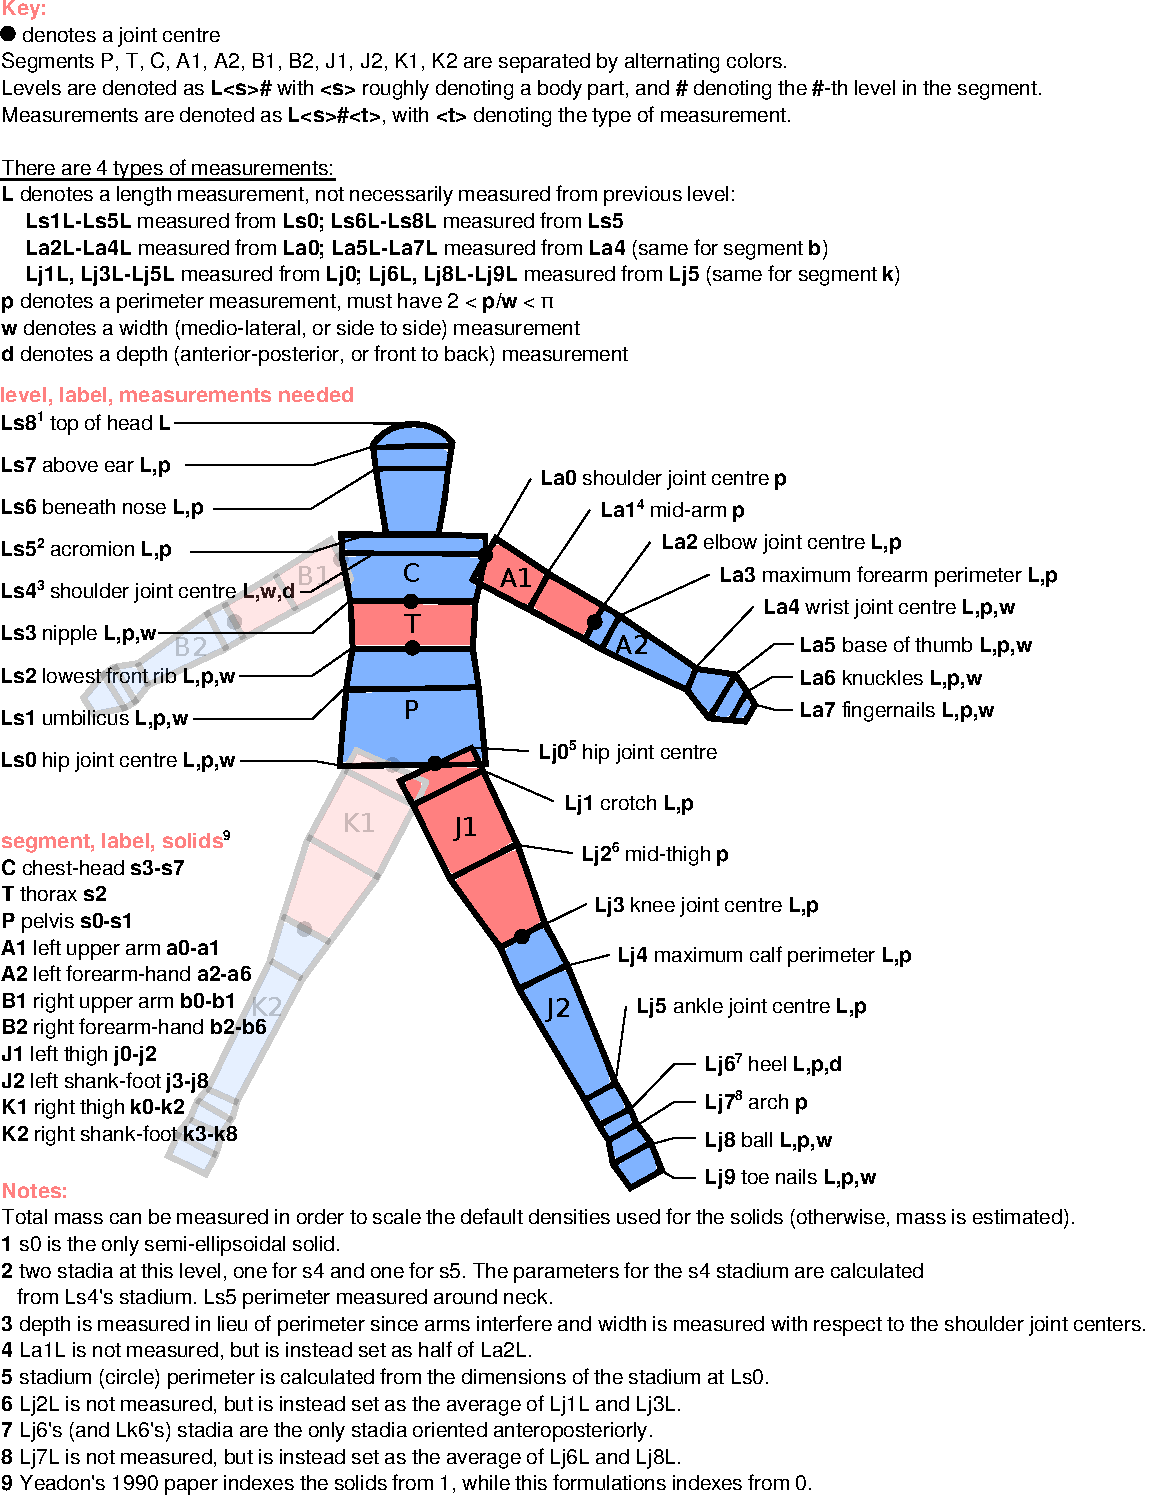
\includegraphics[width=1.6\columnwidth]{figures/measurements.pdf}
  \end{center}
  \caption{
    Measurements required for the human inertia model. The human is defined in
    terms of segments, levels, and solids. Segments are distinguished by
    alternating colors, and are denoted as \textbf{P}, \textbf{A1}, etc. Levels
    are denoted as ``\textbf{L$<$s$>$\#}'', where \textbf{$<$s$>$} denotes a
    segment of the body (e.g. \textbf{j} for the left leg) and \textbf{\#}
    denotes the index of the level in that segment. The solid that is proximal
    to level \textbf{L$<$s$>$\#} is denoted as ``\textbf{$<$s$>$\#}''. The
    model is personalized via 95 measurements of 4 types: lengths \textbf{L}
    along the longitudinal axis of the segments, perimeters \textbf{p} about
    the segments, mediolateral widths \textbf{w}, and anteroposterior depths
    \textbf{d}. Black dots denote joint centers~\cite{Yeadon1990c}.
  }
  \label{fig:meas}
\end{figure*}

\begin{description}
  \item[Segments] The human is assumed to be composed of eleven rigid segments.
    Each of the four limbs has two segments, and the remainder (head and torso)
    consist of three more. Each of these segments is a rigid body, and has at
    least one rotational degree of freedom with respect to the adjacent segment
    to which it is attached. The segments are labeled \textbf{C}, \textbf{A1},
    etc.
  \item[Levels] Each segment is defined by a series of parallel transverse
    cross sections, referred to as levels, both in Yeadon's work and in ours.
    The model contains a total of 45 levels, labeled \textbf{Ls0},
    \textbf{La0}, etc.  Each level has the shape of a \emph{stadium} (see
    Figure \ref{fig:stadium}). A stadium can be defined by any two of the
    following five attributes: its perimeter $p$, radius $r$, thickness $t$,
    width $w$, and depth $d$. However, there are a few situations in which the
    stadium degenerates into a circle. The choice of which two attributes are
    used to define a given stadium depends on its location in the body. For
    example, it is difficult to measure a perimeter around the shoulders
    (\textbf{Ls4}), so a depth is used instead.
  \item[Solids] The inertial properties of each segment are computed by viewing
    each segment as a solid lofted through all the levels in the segment. This
    defines $N-1$ solids in a segment with $N$ levels. The solids are labeled
    \textbf{s0}, \textbf{a0}, etc. All solids in a segment share the same
    longitudinal axis. The shape of a given solid is defined by its two
    bounding stadia and the longitudinal distance between them (the solid's
    height). These are termed \emph{stadium solids}. The only exception is
    \textbf{s7}, the solid above the ear, which is a semi-ellipsoid. The model
    contains a total of 40 solids. Note that in this formulation we begin
    numbering the solids from 0, while Yeadon numbers the solids from 1. This
    is simply to match  Python's 0-based indexing.
\end{description}

\begin{figure}
  \begin{center}
    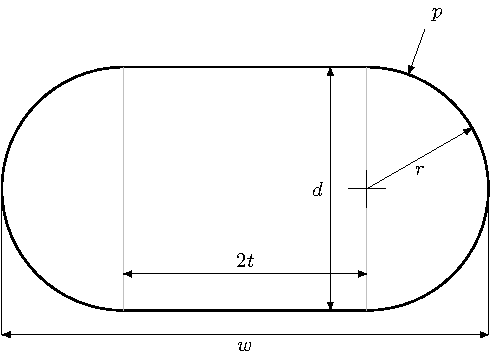
\includegraphics[width=\columnwidth]{figures/stadium.pdf}
  \end{center}
  \caption{
    General stadium cross section shape. The levels that define the segments
    are all in the shape of a stadium, with one exception. A stadium is defined
    by any two of its attributes: perimeter $p$, radius $r$, thickness $t$,
    width $w$, and depth $d$.
  }
  \label{fig:stadium}
\end{figure}

A key feature of this inertia model is that it can be personalized to a given
individual (it is subject specific). The model is personalized via 95
anthropometric measurements. These serve to define each stadium, and to specify
the distances between the stadia (the heights of the stadium solids).

In addition, much of the model's utility comes from the ability to specify the
configuration of the human in which the inertial properties are desired. The
configuration is specified using 21 joint angles between the various segments;
these are described in Figure \ref{fig:config}.

\begin{figure*}
  \begin{center}
    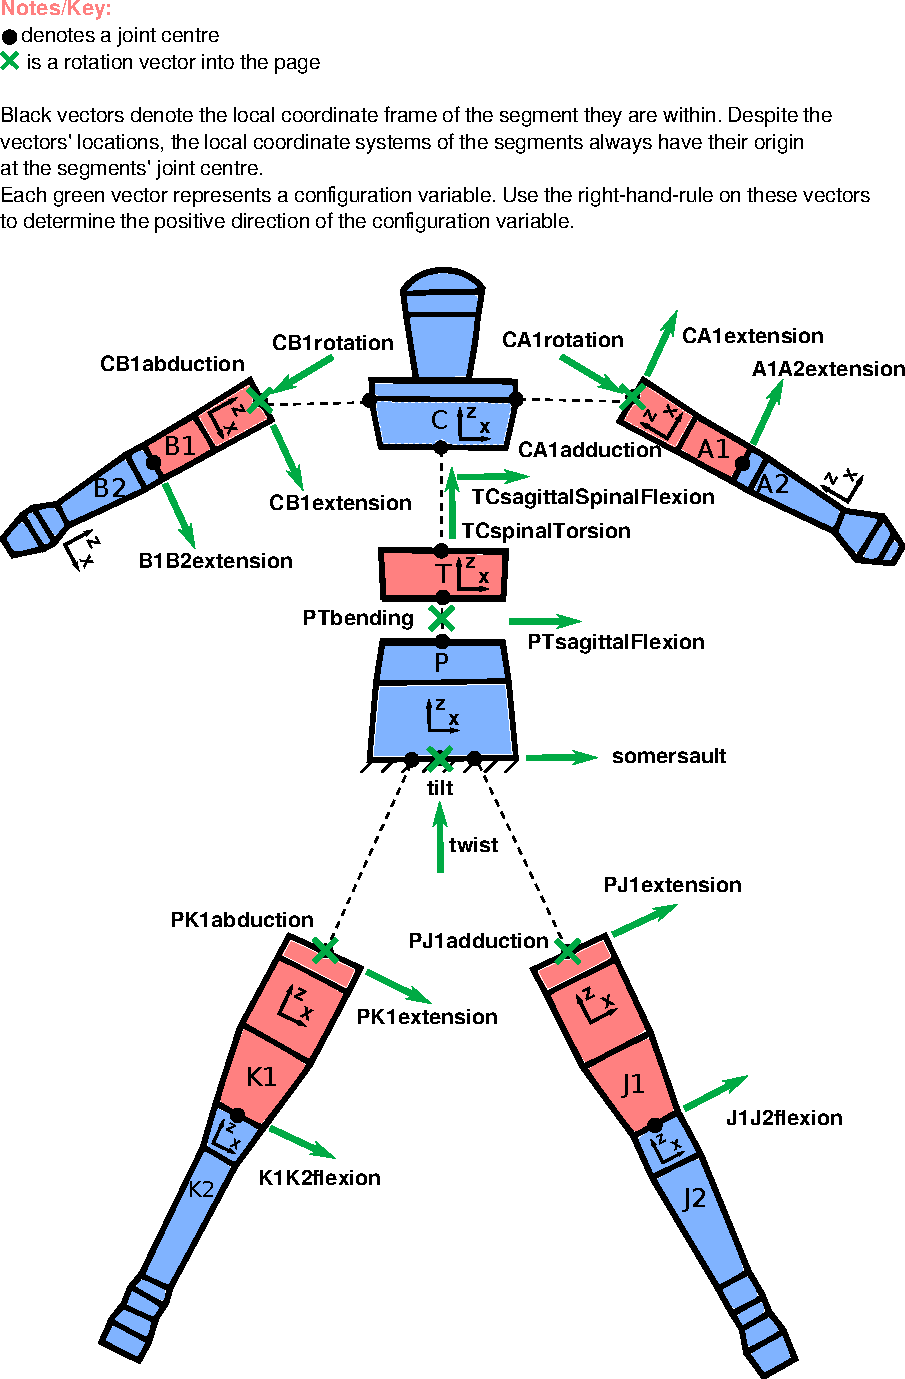
\includegraphics[width=1.6\columnwidth]{figures/configuration.pdf}
  \end{center}
  \caption{
    Configuration variables for the human inertia model. The configuration of
    the human is defined using 21 joint angles, represented by green vectors.
    Green crosses and circles represent vectors into and out of the page,
    respectively. The direction of rotation for a joint angle is given by the
    right-hand rule about its vector. Labels beside the vectors are the names
    of the configuration variables in the code. The black dot on each segment
    denote its joint center. The origin of the fixed coordinate frame is at the
    bottom center of the pelvis segment. The local coordinate frame of each
    segment is specified by the pair of perpendicular black vectors in or next
    to the segments. Despite the locations of these black vectors, the origin
    of a segment's local coordinate system is always at its joint
    center~\cite{Yeadon1990e}.
  }
  \label{fig:config}
\end{figure*}

Thus, Yeadon's model is defined via segments, levels, solids, and configuration
angles. One can personalize the model to an individual using measurements, and
obtain inertial parameters for this individual in any desired configuration.
The only additional data needed are the densities of the solids. We use
Dempster's segmental densities~\cite{Dempster1955} by default, as does Yeadon.
But the user has the option to reassign these to alternative values if desired.
The model is then completed with analytical expressions for a stadium solid's
and semiellipsoid's center of mass location and moments of inertia, using the
parallel axis theorem to combine the inertial properties of multiple stadium
solids. Yeadon provides these explicit formulae in~\cite{Yeadon1990f}. In the
next section, we describe in more detail the measurements required for the
model and the way the configuration is defined.

\section*{Implementation of Yeadon's model}

The previous section makes no departures from Yeadon's work. However, we will
now make some changes that are important for computational implementation and
that serve to generalize his work. These are summarized at the end of this
section.

The experimentalist provides all of the measurements, and optionally the
configuration angles, in two human readable \href{http://yaml.org}{YAML}
formatted text files. The details of these inputs follow.

\subsection*{Measurements}

Measurements are of four types: lengths (\textbf{L}), perimeters (\textbf{p}),
widths (\textbf{w}), and depths (\textbf{d}) and are always tied to a level.
For example, the symbol \textbf{La1p} denotes the perimeter at the \textbf{La1}
level.

Although we require the heights of the individual stadium solids, the
experimentalist does not measure these independently. Instead, measurements are
made of the longitudinal distance across multiple stadium solids. For example,
the \textbf{Ls2L} measurement is not the distance between the \textbf{Ls1} and
\textbf{Ls2} levels. Instead, \textbf{Ls2L} is measured as a distance from
\textbf{Ls0}. To learn the levels from which one measures the various lengths,
see Table \ref{tab:length}.

\begin{table}
  \centering
  \caption{
    \bf{Length measurements}
  }
  \begin{tabular}{cc}
    \hline
    \textbf{length for these levels} & \textbf{are measured from this level}\\
    \hline
    Ls1 - Ls5 & Ls0 \\
    Ls6 - Ls8 & Ls5 \\
    La2 - La4 & La0 \\
    La5 - La7 & La4 \\
    Lb2 - Lb4 & Lb0 \\
    Lb5 - Lb7 & Lb4 \\
    Lj1, Lj3 - Lj5 & Lj0 \\
    Lj8 - Lj9 & Lj5  \\
    Lk1, Lk3 - Lk5 & Lk0 \\
    Lk8 - Lk9 & Lk5  \\
  \end{tabular}
  \begin{flushleft}
    The length measurements are not simply the heights of the stadium solids.
    They are defined relative to a certain preceding level in their segment.
  \end{flushleft}
  \label{tab:length}
\end{table}

There are a few exceptions to the general measurement scheme we have described
thus far. While most of the lengths are  measured directly, some are determined
by other lengths. For example, we set \textbf{La1L} to be half of
\textbf{La2L}, and so the experimentalist does not measure \textbf{La1L}
directly. This means, however, that \textbf{La1p} must be measured halfway down
segment \textbf{A1}. This scenario arises in each limb.

All stadia are oriented mediolaterally except the heels (levels \textbf{Lj6}
and \textbf{Lk6}) which are oriented anteroposteriorily.  Note from Figure
\ref{fig:meas} that one measures a depth at these levels instead of a width.
This depth is in fact the width of a stadium that is rotated through 90
degrees. Other necessary information about exceptions in the measurement scheme
is contained in the notes of Figure \ref{fig:meas}.

Since the densities for the model are provided, we can readily estimate the
human's total mass. However, if the experimentalist measures the mass of the
subject, that mass can be used to proportionally scale all densities in the
model so that the model's total mass matches the subject's measured mass.

\subsection*{Configuration}

In this section we describe, relying heavily on Figure \ref{fig:config}, how
the configuration of the model is implemented. The joint center of each segment
is located with a black dot: it is always located at the center of the base
stadium of the segment. The black arrows on each segment indicate its local
coordinate frame, whose origin is always at the joint center of the segment.
For each segment, the local $z$-axis is the longitudinal axis of the segment.
Each of the green arrows represents a degree of freedom, and indicates the
direction and sign of the corresponding joint angle via the right-hand rule.
Configuration variables are labeled with the names of the two segments at the
joint, and a physiological description of the joint angle. Thus,
\verb+K1K2flexion+ is the right knee flexion angle, and \verb+PK1abduction+ is
the right hip abduction angle (positive for abduction, negative for adduction),
etc. The exceptions to this naming convention are \verb+somersalt+,
\verb+tilt+, and \verb+twist+, which specify the orientation of the \textbf{P}
segment with respect to the fixed coordinate frame.

Most joints enable more than one degree of freedom, but only four have all
three rotational degrees of freedom. Since rotations are not commutative,  we
must specify the order of rotations at multi-degree of freedom joints. Each
child segment is rotated relative to its parent segment using Euler X-Y-Z
angles in a body fixed fashion. Any joints with fewer than three angles follow
this same order, e.g. X-Y.

The default configuration is that in which all configuration variables have a
value of zero. In the default configuration, the local coordinate basis vectors
of all segments align with the global fixed coordinate basis vectors. This
means that for each segment, in the default configuration, the local $x$-axis
lies in a coronal plane and the local $y$-axis is directed posteriorly.
Furthermore, it is assumed that in this configuration, the palms of the hands
face anteriorly.

We now provide the locations of joint centers in our implementation of Yeadon's
model; this information is not in his original papers. The location of the
joint centers of segments \textbf{A1} and \textbf{B1} are at the most distal
points of level \textbf{Ls4} on the respective sides of the body. Joint center
locations for segments \textbf{J1} and \textbf{K1}, respectively denoted as
$\mathbf{p_J}$ and $\mathbf{p_K}$, can be expressed in the local coordinate
frame of the pelvis \textbf{P}:

\begin{align}
    \mathbf{p_J} &= \frac{1}{2} (t_{Ls0} + r_{Ls0})\hat{\mathbf{i}} \\
    \mathbf{p_K} &= -\frac{1}{2} (t_{Ls0} + r_{Ls0})\hat{\mathbf{i}},
\end{align}
where $\hat{\mathbf{i}}$ is a unit vector along the $x$-axis of the pelvis,
$t_{Ls0}$ is the thickness of the stadium at level \textbf{Ls0} and $r_{Ls0}$
is its radius. This choice is informed by calculations present in the ISEG code
published in~\cite{Yeadon1984a}. Joint center locations in all other segments
are at the center of the last stadium in the preceding segment.

\subsection*{Departures from Yeadon's work}

There are a few ways in which our implementation of the human inertia model
differs from that presented in~\cite{Yeadon1990c, Yeadon1990f, Yeadon1990e,
Yeadon1990d}. Some of these differences arise from the fact that his work was
tailored for aerial movement, more specifically for twisting somersaults. We
expect, however, that our implementation of the model can be used in a more
general set of investigations.

\begin{description}
    \item[Symmetry of limbs] Yeadon averages the measurements for the left and
      right limbs so that the model is symmetric. We provide the user with the
      option of imposing this symmetry, but the averaging is not performed by
      default.
    \item[Acromion stadia] One can see that there are actually two different
      cross sections at the acromion level \textbf{Ls5}: we use the wider one
      for solid \textbf{s4} in the chest and the thinner one (actually, a
      circle) for solid \textbf{s5} in the head. The perimeter measurement at
      \textbf{Ls5} is used for the bottom of \textbf{s5}. In our
      implementation, the stadium at the top of \textbf{s4} is determined
      internally by the \textbf{Ls4} stadium by:
      \begin{align}
        r &= 0.57 r_{Ls4} \\
        t &= \frac{1}{2}w_{Ls4} - r
      \end{align}
      where $r$ and $t$ are the radius and thickness for the top stadium of
      \textbf{s4}, respectively, and $r_{Ls4}$ and $w_{Ls4}$ are the radius and
      width of the stadium at level \textbf{Ls4}, respectively.  This issue is
      not addressed in ~\cite{Yeadon1990c, Yeadon1990f, Yeadon1990e,
      Yeadon1990d}, and our implementation disagrees with the ISEG code found
      in ~\cite{Yeadon1984a} (see page 358 line 251). The justification for our
      choice is to agree with a more recent version of Yeadon's code, provided
      to us in a personal communication.
    \item[Hip joint center stadia in the thigh] The experimentalist makes no
      measurements at the \textbf{Lj0} or \textbf{Lk0} stadia, though these
      stadia must be defined to define solids \textbf{j0} and \textbf{k0}. In
      our implementation, these stadia are circles with the same radius $r$:
      \begin{equation}
        r = \frac{1}{2}\sqrt{r_{Ls0} w_{Ls0}}
      \end{equation}
      where $r_{Ls0}$ and $w_{Ls0}$ are the radius and width of the
      \textbf{Ls0} stadium, respectively. As with the acromion stadia mentioned
      above, the justification is that this has been implemented in the more
      recent version of the code shared with us.
    \item[Relationships between configuration variables] Yeadon enforced
      relationships between certain configuration variables, such as symmetric
      movement of the legs with respect to the pelvis. We neither assume nor
      impose any relationships between the 21 configuration variables; all are
      independent. As a result our model allows the body to assume any
      geometrically feasible configuration with physiological bounds.
    \item[Inconsistent measurements] The ratio of a stadium's perimeter to its
      width must be greater than 2 and less than $\pi$. If the measurements do
      not satisfy these constraints, then the stadium is assumed to be a
      circle. This scenario is not discussed by Yeadon.
    \item[Degenerate stadia] In the case where a stadium has zero thickness (a
      circle), the stadium is degenerate and some equations have a zero in the
      denominator. In this scenario, Yeadon still employs the formulae for
      stadium solids but sets the thickness to be very
      small~\cite{Yeadon1990f}.  Instead, we manipulate the equations so that
      the approximation is not necessary.
    \item[Joint center of chest-head segment] We locate the joint center
      between the torso \textbf{T} and the chest-head \textbf{C} at the center
      of level \textbf{Ls3}. This is in accordance with Figure 1 of
      \cite{Yeadon1990e}. However, this is a departure from
      ~\cite{Yeadon1984a}, in which the joint center of the chest-head is
      placed at the midpoint of the shoulder joint centers.
\end{description}

\section*{Software design}

We implemented the inertia model in the Python language as a package named
\verb+yeadon+.  Python was chosen due to its ease of use, wide adoption, its
stable infrastructure for distributing open source software, and its strong
scientific community (\href{http://www.scipy.org}{SciPy}).

The input to \verb+yeadon+ consists of (1) geometric measurements of a subject,
and (2) joint configuration angles. Using these two inputs, the inertial
properties of the subject in this configuration can be calculated.

The \verb+yeadon+ package contains 5 modules: \verb+human+, \verb+segment+,
\verb+solid+, \verb+ui+, and \verb+gui+. The \verb+human+ module contains the
public interface of the package, and the \verb+segment+ and \verb+solid+
modules are used internally to construct objects available in the \verb+human+
module. The user interacts either directly with the \verb+human+ module, or via
the \verb+ui+ or \verb+gui+ modules, both of which are clients to the
\verb+human+ module. The \verb+human+ module contains only the \verb+Human+
class, the \verb+segment+ module contains only the \verb+Segment+ class, and
the \verb+solid+ module contains the \verb+Stadium+, \verb+Solid+,
\verb+StadiumSolid+, and \verb+Semiellipsoid+ classes. The package relies
heavily on composition. The \verb+Human+ constructor constructs all
\verb+Stadium+'s, \verb+Solid+'s, and \verb+Segment+'s, and ties together these
objects appropriately. A visual description of the class hierarchy is shown in
the UML diagram in Figure \ref{fig:umldiagram}.

\begin{figure}
  \begin{center}
    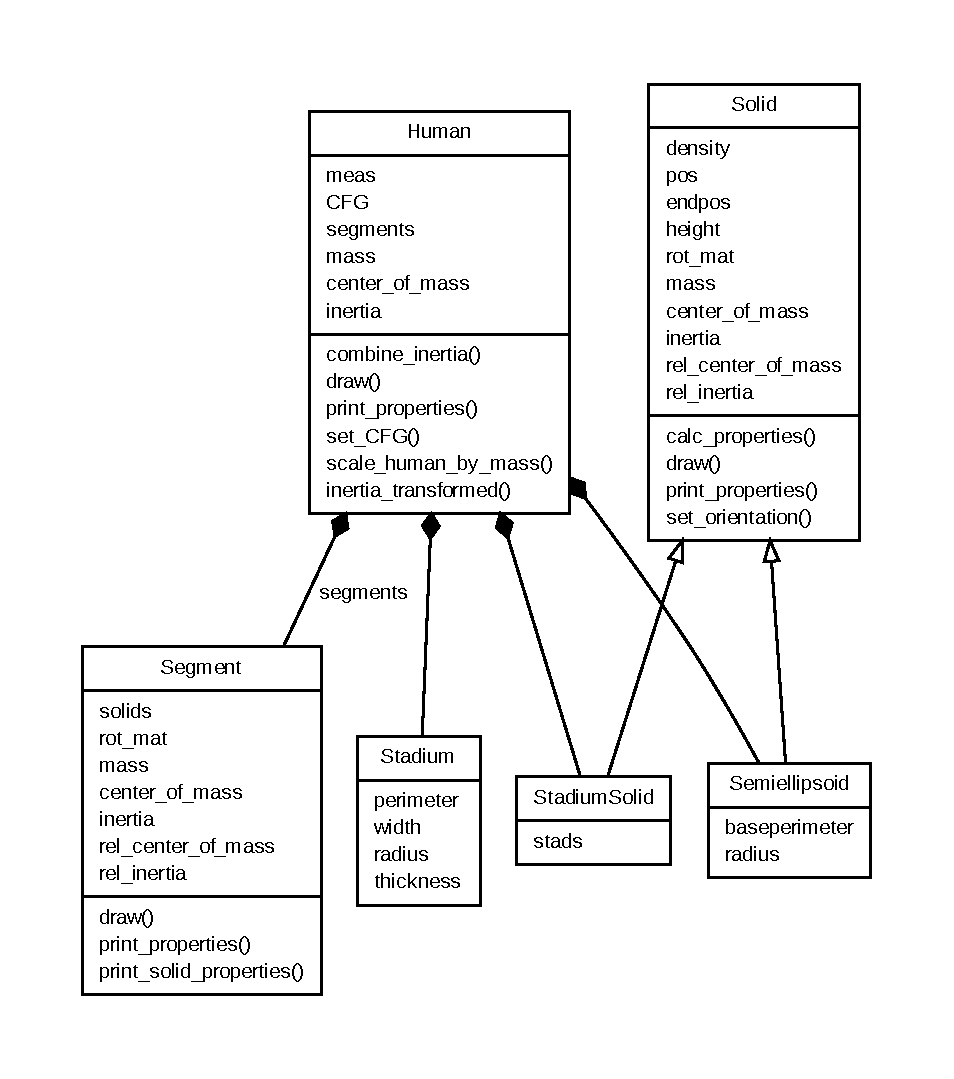
\includegraphics[width=\columnwidth]{figures/umldiagram.pdf}
  \end{center}
  \cprotect\caption{
    UML diagram of Yeadon package.  The \verb+Human+ class constructs all
    \verb+Segment+'s, \verb+Solid+'s, and \verb+Stadium+'s, and assembles them
    appropriately. The classes \verb+StadiumSolid+ and \verb+Semiellipsoid+
    inherit from \verb+Solid+.  This diagram does not reveal the entire public
    interface of the classes shown. The user interacts with the software
    through the attributes or methods of the \verb+Human+ class, or via the
    \verb+ui+ or \verb+gui+ modules.
  }
  \label{fig:umldiagram}
\end{figure}

The GUI is built using Mayavi~\cite{Ramachandran2011} which is both a high
level Python interface to the Visualization Tool Kit~\cite{Schroeder2006} and a
lightweight application framework. We utilized Mayavi's ability to rapidly
create cross platform graphical interfaces to expose the underlying
\verb+yeadon+ classes through interactive widgets. The graphical user interface
shown in Figure \ref{fig:gui} allows the user to load measurement data files,
adjust configuration variables interactively, view the human body's mass center
location, visualize its inertia ellipsoid, and view the resulting whole-body
inertial properties.

\begin{figure*}
  \begin{center}
    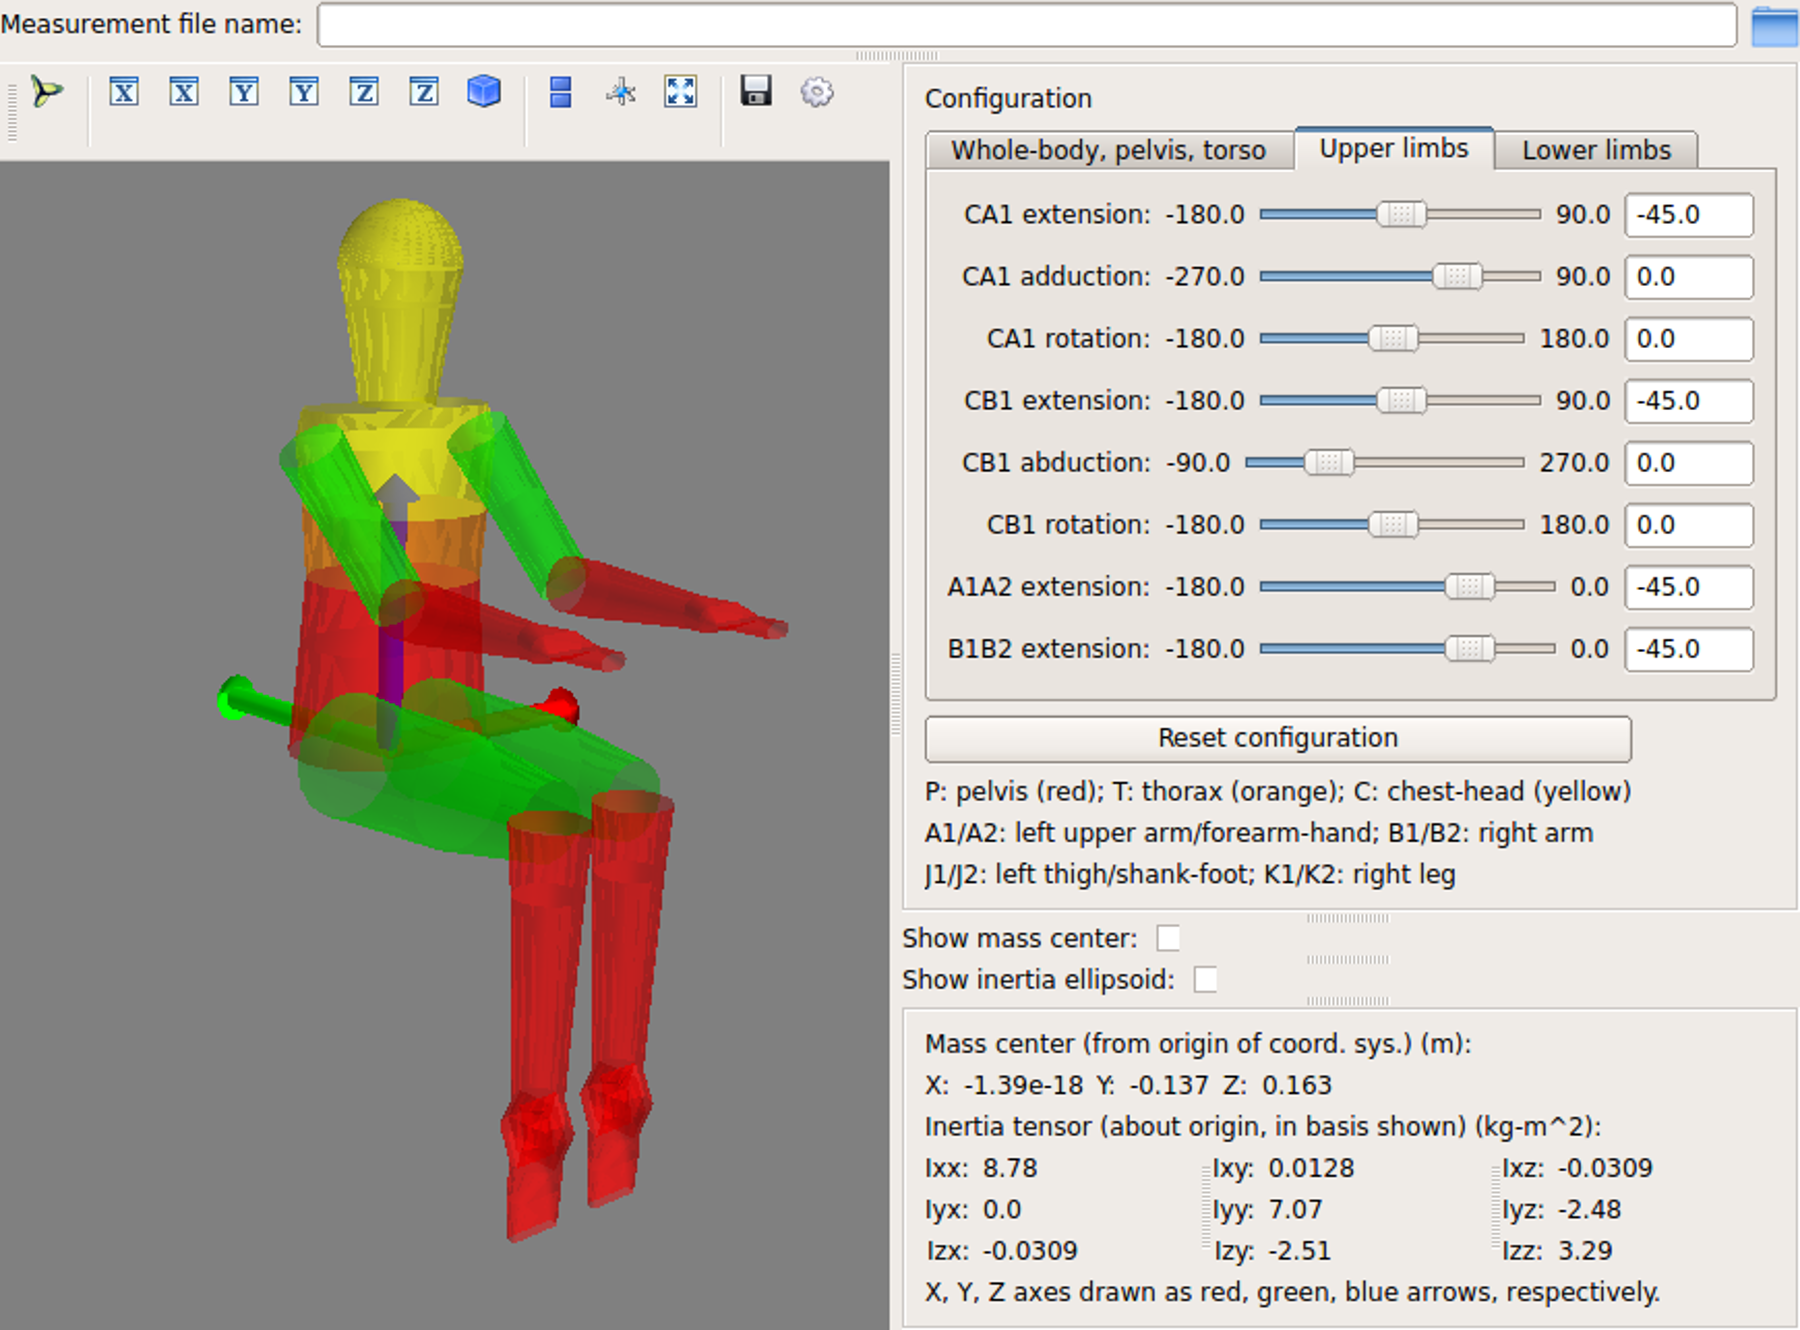
\includegraphics{figures/gui-screenshot.png}
  \end{center}
  \caption{
    Screenshot of the GUI application. A screenshot of the Mayavi GUI
    application (QT backend) running on Ubuntu 14.04 is shown. The user can
    supply the path to measurement YAML files to obtain inertial properties for
    a specific subject. The graphics window on the left shows a 3D view of the
    model. The viewing angle, camera perspective, and other details can be
    manipulated with a mouse or from the toolbar above the window. Tabs on the
    right provide sliders and text inputs for all 21 configuration variables
    and allow the user to interactively set the configuration. The ``Reset
    Configuration'' button sets all the configuration variables to zero. The
    mass center and inertia ellipsoid for the entire body can be toggled with
    the checkboxes. Finally, the whole-body mass, center of mass coordinates,
    and inertia tensor are displayed in the bottom right and are updated
    interactively as the configuration is altered.
  }
  \label{fig:gui}
\end{figure*}

The primary outputs of the software include:

\begin{itemize}
  \item Whole-body inertial properties of the model in any given configuration
    with respect to any point and reference frame.
  \item Segment-fixed inertial properties for any single solid or any
    combination of solids.
  \item Visual depiction of the model in a given configuration. These can be
    exported to bitmap files.
\end{itemize}

The software provides inertial properties (mass, center of mass location, and
moments of inertia) for the whole human, for an individual segment, for an
individual solid, or for any combination of segments and solids. In the first
case of the whole human, center of mass locations and moments of inertia are
expressed in the global coordinate frame. This frame has its origin at the
bottom center of solid \textbf{s0}, and is aligned with the local frame of
segment \textbf{P} when \verb+somersalt+, \verb+tilt+, and \verb+twist+ are
zero. In the cases of individual segments or solids, inertial properties are
expressed in either the local frame of the particular segment or in the fixed
frame. Inertial properties for any other combination are expressed in the fixed
frame.

\section*{Usage}
\label{sec:usage}

We begin our description of how one uses \verb+yeadon+ with an example of an
ice skater performing a spin. As is commonly taught in high school physics, an
ice skater can change his angular velocity by altering their moment of inertia
due to conservation of angular momentum. By what factor can an ice skater
increase his angular velocity by bringing in his arms? The commands in Figure
\ref{fig:ice-skate-code} perform this calculation.

\begin{figure*}
  \begin{verbatim}
    >>> import yeadon
    >>> pi = 3.14159
    >>> # Load a prepared measurements file.
    >>> h = yeadon.Human('male1.txt')
    >>> # Create a 3D rendering of the model.
    >>> h.draw()
    >>> # Print the moment inertia about the global Z axis.
    >>> print('Arms down: {:.2f} kg-m^2'.format(h.inertia[2, 2])
    Arms down: 0.55 kg-m^2
    >>> # Set the configuration of the shoulder angle.
    >>> h.set_CFG('CA1adduction', -0.5 * pi)
    >>> h.set_CFG('CB1abduction', 0.5 * pi)
    >>> # Print the updated moment inertia about the global Z axis.
    >>> print('Arms out: {:.2f} kg-m^2'.format(h.inertia[2, 2]))
    Arms out: 1.58 kg-m^2
  \end{verbatim}
  \caption{Python interpreter session showing how one could compute the spin
    moment of inertia of an ice skater in two configurations.
  }
  \label{fig:ice-skate-code}
\end{figure*}

The subject represented by the measurements in \verb+male1.txt+ can increase
his angular velocity (about the vertical axis) by a factor of 2.9 by bringing
the arms in toward the body from an extended position. Figure
\ref{fig:iceskater} shows a rendering of a human in a more complicated and
asymmetrical ice skating spin pose to demonstrate that the model is capable of
complex configurations. We can also obtain the mass and center of mass location
of the whole human with the code presented in Figure \ref{fig:mass-com-code}.

\begin{figure}
  \begin{verbatim}
    >>> h.mass
    58.200488588422544
    >>> h.center_of_mass
    array([[ -9.53791842e-19],
           [  0.00000000e+00],
           [  3.77172308e-02]])
  \end{verbatim}
  \caption{Python interpreter session demonstrating accessing the attributes
  for mass and center of mass.}
  \label{fig:mass-com-code}
\end{figure}

\begin{figure}
  \begin{center}
    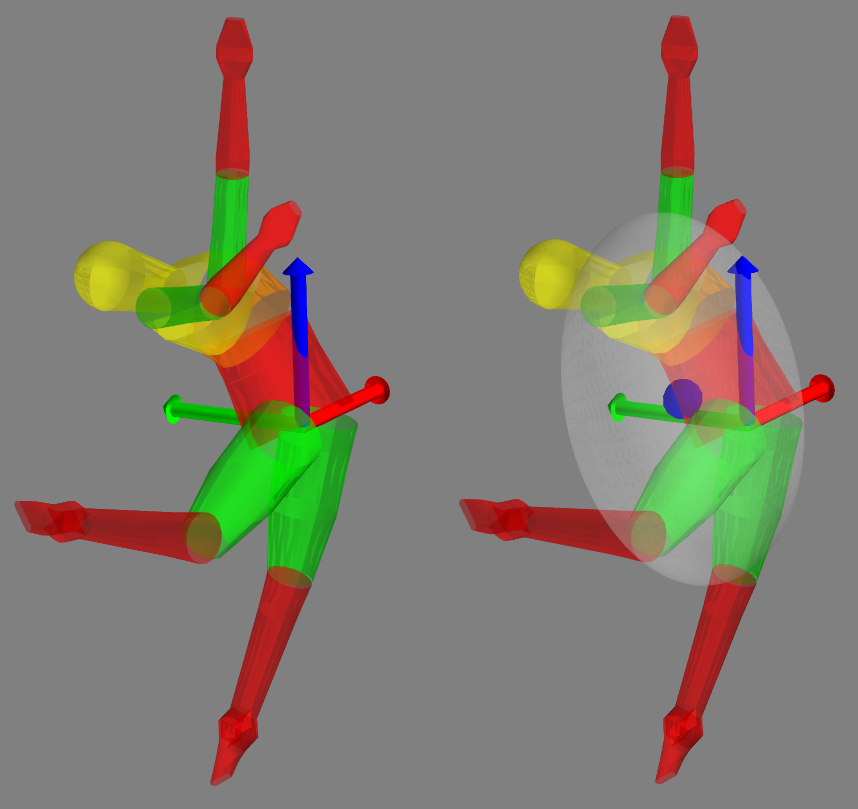
\includegraphics[width=\columnwidth]{figures/ice-skater-double.png}
  \end{center}
  \caption{View of the ice skater model in an asymmetrical spin pose. An ice
    skater can increase the axial moment of inertia by extending their limbs
    away from the spin axis. The right image shows both the center of mass
    sphere and the inertia ellipsoid for this pose. Note that the center of
    mass is actually outside of the body for the gravitational force resultant
    to be directed through the ground contact point.
  }
  \label{fig:iceskater}
\end{figure}

With a measurement of the subject's actual mass, we can scale all the segmental
densities so that \verb+h.mass+ is the same as our experimentally measured
mass; see Figure \ref{fig:mass-scale-code}:

\begin{figure*}
  \begin{verbatim}
    >>> # Print the mass of the left leg.
    >>> h.K1.mass
    8.5047753220376521
    >>> # Scale the density values based on the measured mass.
    >>> h.scale_human_by_mass(60.0)
    >>> # The overall mass is updated.
    >>> h.mass
    60.0
    >>> # A slight increase in the segment mass can be seen.
    >>> h.K1.mass
    8.767736005291324
  \end{verbatim}
  \caption{Python interpreter session which demonstrates segment density
  scaling.}
  \label{fig:mass-scale-code}
\end{figure*}

It is also possible to calculate the combined inertia properties of various
segments and/or solids. For example, we can obtain the mass, center of mass
location, and inertia tensor of the entire right arm via the code in Figure
\ref{fig:combine-inertia-code}.

\begin{figure*}
  \begin{verbatim}
    >>> # Generate the mass, center of mass, and inertia tensor for the right arm.
    >>> h.combine_inertia(['B1', 'B2'])
    Combining segments/solids ['B1', 'B2'].
    (2.8193675676892624,
     array([[-0.1515    ],
            [ 0.        ],
            [ 0.19831659]]),
     matrix([[ 0.09098096,  0.        ,  0.        ],
             [ 0.        ,  0.09110269,  0.        ],
             [ 0.        ,  0.        ,  0.00194811]]))
    \end{verbatim}
    \caption{Python interpreter sessions which demonstrates collecting inertial
    properties of multiple segments.}
    \label{fig:combine-inertia-code}
\end{figure*}

All of the methods have rich docstrings accessible via the Python \verb+help()+
function. For example the previous method's docstring shows the three returned
values in Figure \ref{fig:docstring}.

\begin{figure*}
  \begin{verbatim}
    >>> help(h.combine_inertia)
    Returns the inertia properties of a combination of solids
    and/or segments of the human, using the fixed human frame (or the
    modified fixed frame as given by the user). Be careful with inputs:
    do not specify a solid that is part of a segment that you have also
    specified. This method does not assign anything to any object
    attributes (it is 'const'), it simply returns the desired quantities.

    See documentation for description of the global frame.

    Parameters
    ----------
    objlist : tuple
        Tuple of strings that identify a solid or segment. The
        strings can be any of the following:

        * solids: 's0' through 's7', 'a0' through 'a6', 'b0' through 'b6',
          'j0' through 'j8', 'k0' through 'k8'
        * segments: 'P', 'T', 'C', 'A1', 'A2', 'B1', 'B2', 'J1', 'J2',
          'K1', 'K2'

    Returns
    -------
    combined_mass : float
        Sum of the masses of the input solids and/or segments.
    combined_COM : np.array (3,1)
        Position of the center of mass of the input solids and/or segments,
        expressed in the global frame .
    combined_inertia : np.matrix (3,3)
        Inertia tensor about the combined_COM, expressed in the global frame.
  \end{verbatim}
  \cprotect\caption{An example docstring for a method in the \verb+Human+ class.}
  \label{fig:docstring}
\end{figure*}

\section*{Advanced Example}
\label{sec:advanced-example}

This software was originally developed as part of an effort to easily compute
the inertial properties of a human rider seated on a bicycle. A common way to
model the bicycle/rider dynamics is to assume that the rider is rigid and fixed
to the bicycle rear frame ~\cite{Meijaard2007a}. Our studies~\cite{Moore2012}
included a variety of bicycles and riders, for which various combinations of
the inertial properties of the bicycle rear frame and rider were required.

As an advanced example, we will configure the model using the \verb+yeadon+
software such that the human is seated on the bicycle, feet at the bottom
bracket axis, and hands on the handlebars with arms hanging down. The inertia
of the human will be computed first with respect to its center of mass and then
combined with that of the bicycle rear frame  using the parallel axis theorem
to give the total inertia of the human rigidly affixed to the bicycle rear
frame in the bicycle's reference frame.

We use the definitions and parameters of the benchmark bicycle model
\cite{Meijaard2007a} defined using the standard SAE vehicle coordinate system
(which is different from Yeadon's coordinate system). In addition to the
geometrical parameters in the benchmark bicycle, the bicycle rear frame and
handlebar location are defined by several geometric and inertial parameters.
Furthermore, a single measurement of the rider's forward lean angle relative to
the bicycle frame was made.

An interactive IPython~\cite{Perez2007} notebook in the supplementary materials
provides a detailed walk through this advanced example. This example is also
included in the Yeadon 1.2.0 software source files and a
\href{http://nbviewer.ipython.org/github/chrisdembia/yeadon/blob/v1.2.0/examples/bicyclerider/bicycle_example.ipynb}{rendered
  version is viewable with NBViewer}. The following briefly summarizes the
steps involved in the computation and further illustrates use of the
\verb+yeadon+ software.

\begin{enumerate}
  \item Geometric and inertial properties of the bicycle were estimated with an
    independent method~\cite{Moore2012}. Inertial properties of the rear frame
    of the bicycle were expressed in the SAE coordinate system described above.
  \item We solve for a configuration of the human that enforces the human rider
    to be seated properly on the bicycle, for any bicycle. The SymPy Mechanics
    package~\cite{Gede2013} is used for these computations.
  \item The \verb+Human.inertia_transformed+ method is used to express the
    human's inertia in the bicycle's reference frame.
  \item The combined mass and center of mass location of the human and the rear
    frame of the bicycle are computed and the parallel axis theorem is employed
    to express the moments of inertia of each body about the combined center of
    mass, where they are then summed to get the combined moments of inertia.
\end{enumerate}

The example shows how to set a complex configuration of the Yeadon model and
extract the geometric and inertial properties expressed in arbitrary reference
frames and relative to arbitrary points as well as how to visualize the
configuration.

\section*{Software Availability}
The software is distributed as the \verb+yeadon+ package on the Python Package
Index at \url{http://pypi.python.org/pypi/yeadon/} under the
\href{http://opensource.org/licenses/BSD-3-Clause}{3 clause BSD license} which
permits both non-commercial and commercial use.  The software development is
currently managed and hosted at GitHub
(\url{http://www.github.com/chrisdembia/yeadon}). This paper corresponds to the
1.2.0 release of the software \cite{Christopher:11579}. Furthermore, online
documentation including both prose description and the API docstrings is
included with the source code and can also be viewed at
\url{http://yeadon.readthedocs.org}.

\section*{Conclusion}
We have presented an open source software package that implements a widely used
inertial model of a human. This package is available in public repositories
under a permissive copyright license. The software provides an API for use as a
library, and also has both a command-line user interface and a graphical user
interface for interactive high level use as a standalone application. The
structural design of the software is presented as an introduction to the source
code which is available in a public repository that is open for contributions
and modifications. Finally, we have described both simple and advanced use
cases for the API, one in the text of the paper and one in the supplementary
IPython notebook.

\subsection*{Author contributions}
J.K.M and M.H. conceived of the software tool. C.D. was the primary developer
of the software and primary author of the documentation and the paper. J.K.M
contributed to the development of the software and authorship of the
documentation and the paper.  M.H. advised the project and contributed to the
writing of the paper. C.D and J.K.M prepared the first draft of the manuscript.
All authors were involved in the revision of the draft manuscript and have
agreed to the final content.

\subsection*{Competing interests}
The authors have no  financial, personal, or professional competing interests
that could be construed to unduly influence the content of this article.

\subsection*{Grant information}
This material is partially based upon work supported by the National Science
Foundation under Grant No. 0928339. Any opinions, findings, and conclusions or
recommendations expressed in this material are those of the authors and do not
necessarily reflect the views of the National Science Foundation.

\subsection*{Acknowledgements}
We thank M.R. Yeadon for sharing his source code and measurement methodologies.
His generosity has greatly improved the quality of our software.

{\small\bibliographystyle{unsrt}
\bibliography{humaninertia}}

% When all authors are happy with the paper, use the
% ‘Submit to F1000Research' button from the Share menu above
% to submit directly to the open life science journal F1000Research.

% Please note that this template results in a draft pre-submission PDF document.
% Articles will be professionally typeset when accepted for publication.

% We hope you find the F1000Research writeLaTeX template useful,
% please let us know if you have any feedback using the help menu above.

\end{document}
